% Intended to be compiled with XeLaTeX

\documentclass[11pt,letterpaper]{article}

\usepackage{graphicx}
\usepackage{natbib}
\usepackage{fullpage}
\usepackage{lineno}
\usepackage{multirow}
%\usepackage{wrapfig}
\usepackage{amsmath}
\usepackage{amssymb}
%\usepackage{sidecap}
\usepackage{hyperref}
\usepackage{bibentry}
\nobibliography*

\begin{document}

\setlength{\parindent}{0mm}
\setlength{\parskip}{0.4cm}

\bibliographystyle{apalike}

%\modulolinenumbers[5]
%\linenumbers

\title{\textbf{GEMINI} Implementation Details}
\author{Matthew D. Zettergren, PhD\\ \texttt{matthew.zettergren@icloud.com}}
\maketitle

\tableofcontents

\pagebreak

\section{GEMINI Model:  Executive Summary}

\textbf{GEMINI:}  The ``\underline{G}eospace \underline{E}nvironment \underline{M}odel for \underline{I}on-\underline{N}eutral \underline{I}nteractions'' is a 3D ionospheric model based on \citet{Zettergren:2012}, that has been applied in wide variety of ionospheric studies (Zettergren, op.\ cit.).  The model uses a tilted dipole \citep{Huba:2000} or Cartesian mesh, and comprises a fluid system of equations \citep{Schunk:1977,Blelly:1993} describing dynamics of the ionospheric plasma, self-consistently coupled to a quasi-static (defined below) treatment of electrical currents. The fluid system is a set of three conservation equations (mass, parallel momentum, and energy) for each ionospheric species \citep[][ Appendix A]{Zettergren:2015}.  Source terms in the continuity equations include photoionization \citet{Solomon:2005,Richards:1994} and impact ionization via integration of the physics-based energetic electron transport model, GLOW \citep{Solomon:2001}.  Efficient semi-empirical methods for energy deposition calculations \citep{Fang:2008} can also be used.  A full set of chemical reactions needed for the E- and F-regions is taken from \citet[][]{Diloy:1996,StMaurice:1998}.

Perpendicular components of the plasma momentum equations in GEMINI are resolved via a quasi-static force balance approximation \citep{Zettergren:2015b}, viz. a static solution is applied but the parameters of the system  (importantly conductivity) are allowed to change in time.  Electric fields are found by enforcing a divergence-free current density, where the current consists of conduction, polarization, and pressure contributions \citep[e.g. as in][]{Kintner:1985}. This approach assumes a leading order electrostatic description supplemented by terms correcting for polarization currents from varying field structures \citep{Mitchell:1985} (i.e. ion inertial effects).  Because the GEMINI solver is inherently (quasi-)static in nature it can be driven from either field-aligned current (FAC) or electric field conditions boundary conditions.  Specifically, the ionospheric electric field is approximated by $\mathbf{E}=-\nabla \Phi$ but current closure solutions include ion inertial effects.  
\begin{figure}
  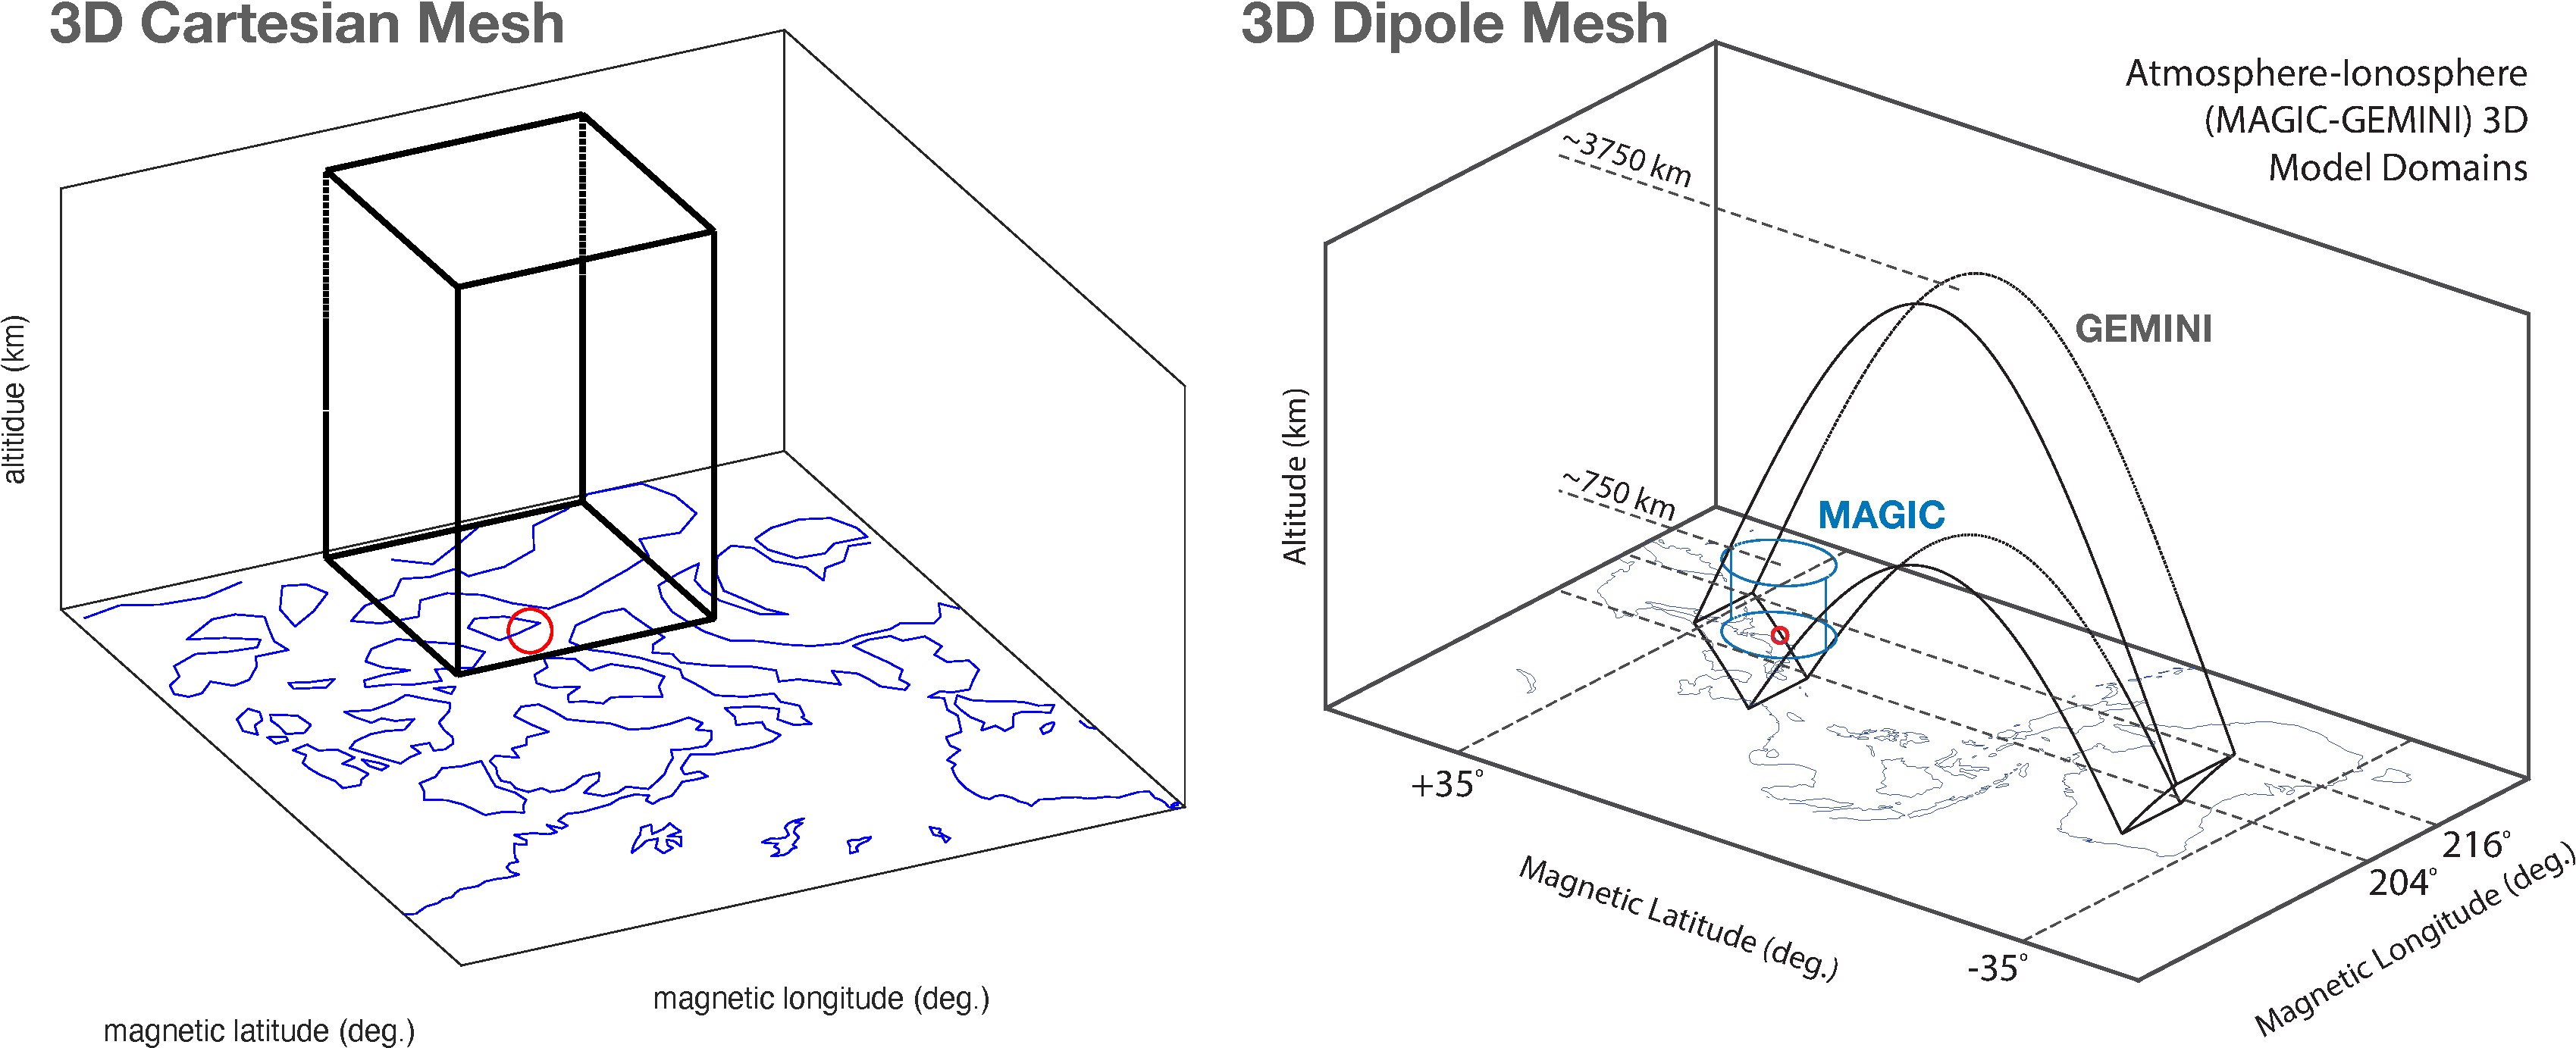
\includegraphics[width=\textwidth]{./figures/GEMINI_mesh-crop.pdf}
  \caption{Examples of commonly used GEMINI mesh configurations: (left) a Cartesian mesh centered near the geomagnetic pole near Resolute Bay Canada, (right) an interhemispheric dipole mesh used with studies of infrasound and gravity wave impacts on the ionosphere.  }
  \label{fig:GEMINI}
\end{figure}

The use of a quasi-static solution notably omits Alfv\'en waves; however, many mesoscale structures are well-described as static \citep[e.g.][]{Lynch:2015}.  Recent reviews suggest that alternating current (AC) Poynting flux is typically reported at lower levels than direct current (DC) Poynting flux, but can be highly variable; the relative importance of these two sources (DC vs. AC) is unknown \citep{Kaeppler:2022}.  Our modeling focuses on the DC input effects (and particle inputs) as we argue this is the only part of the Poynting flux that can feasibly be captured by non-idealized models -- resolving propagation of Alfv\'en waves in a cross-scale (meso-to-large), 3D ionosphere-thermosphere (plasma-neutral coupling) model is computationally infeasible for resolutions and grid extents that we target.   At the very minimum, research suggests that the DC part of the incoming energy and momentum (stress) is a major (perhaps even the largest) contributor and our data-driven methodology permits us to evaluate the extent to which the observations are DC.  As better computational resources and algorithms become available in the future it should be possible to begin to address AC portions of the spectrum, but that is not within the project scope.  

%% MZ - cut to save space
GEMINI presently assumes that the geomagnetic field lines are equipotentials (a particularly good assumption for highly conducting situations likely to accompany precipitation) and employs a field line integration in the equation solved to describe conservation of charge \citep[cf.][Equation 1]{Zettergren:2015}.  Newer versions of GEMINI also include additional current terms needed for high-resolution modeling, like diamagnetic currents and diffusive transport perpendicular to $\mathbf{B}$. 

\section{Cmake Build System for GEMINI}

\emph{MH - focus on current state and additions made during AIRWaveS}



\section{}



\section{Continuous Integration (CI)}

\subsection{Automatic CI}

The base \texttt{gemini3d} repository includes a set of integration and unit tests that can be run by a user upon compilation of model to test a number of model components as well as several integration tests that run simple model configurations and compare results against reference data archived in online repositories.  These tests are also run via GitHub Actions anything a new update is pushed to the \texttt{gemini3d} repository.  These test are designed to be able to run in a matter of minutes on a modest computer.  

\emph{MH:  cmake implementation details, locations of reference data, details of github actions and examples, descriptions of tests}

\emph{example plots of output?}

\subsection{Comprehensive Continuous Integration (long CI)}

Integration tests done by the automatic CI system are necessarily limited to those which can run quickly; yet there are a huge number of potential applications of the GEMINI model.  A more comprehensive set of tests, in the \texttt{gemci} repository have been developed in order to check a number of other common use cases of the model against reference data.  These include:
\begin{itemize}
  \item Instability development utilizing periodic grids and quasi-dynamic solvers:  
  \item Auroral electron precipitation and field-aligned currents:  
  \item 2D and 3D cusp, open curvilinear grids with soft electron precpitation and field-algned:   currents
  \item Closed, dipole grids with file input neutral perturbations:  
\end{itemize}
A more comlpete description of each of these tests is given in the README file in the \texttt{gemci} repository under the \texttt{cfg} folder.  The complete set of long CI tests is designed to be run in about 12 hours on a modest computer system.  

\emph{MH:  cmake implementation details, locations of ref. data}

\emph{example plots of output?}



\section{GEMINI Data Structures}

\subsection{Mesh Objects}

\subsection{Inputdata Objects}



\section{\texttt{libgemini}}

To allow maximum flexibility in how GEMINI functionality is used, we have developed a library containing core functionality that is accessible from applications written in fortran, C, and C++ languages.  

\emph{MZ - Modularization of app-level implementation from numerical operations}

\emph{MZ - Isolation of grid and solution data; toward allowing multiple patches on a single worker}.  There is a need in some applications for GEMINI to accommodate multiple independent sub-domains (with attendant grid and solution data) on a single mpi worker.  This precludes use of any module-scope variables as these are limited to one per worker and required a full code refactor so that grid and solution data are always passed to numerical routines as procedure arguments (and not thru common blocks or module-scope variables).  

\emph{MZ - C interoperability details}



\section{\texttt{trees-GEMINI}}

A GEMINI application has been implemented under the forestclaw API in order to allow adaptive mesh refinement (AMR) using forestclaw's three-dimensional, extruded mesh capabilities.  EMINI applications using ForestClaw / p4est AMR, termed Trees-GEMINI, have recently been developed as part of Phase 1 of DARPA's AtmoSense program.  Our current setup uses GEMINI with an ``extruded'' mesh, whereby the AMR is done in two dimensions while the full extent of the third dimension is held on each computational ``patch''.  In Trees-GEMINI the extruded dimension is along geomagnetic field line which allows us to use existing implicit solvers for the numerically stiff electron thermal conduction process.  Such solvers require all data along the parallel coordinate at once to function but are capable of dealing with the fast thermal conduction time scales (in the electron population) while maintaining an otherwise reasonable time step for other explicit solutions for transport.  Figure \ref{fig:Trees-GEMINI} shows a Trees-GEMINI simulation using multiply refined regions to model low-frequency acoustic wave propagation through the ionosphere using input from the MAGIC atmospheric dynamics model.  

Trees-GEMINI currently contains most of the functionality of the core libGEMINI libraries including input data handling, dipole and Cartesian meshes, specifications of boundary conditions, fluid plasma solvers (chemistry, advection, diffusion), photoionization and impact ionization solvers, along with new output routines to optionally generate \texttt{vtk/vtu} files for efficient 3D visualization via the Paraview multi-platform open source application (Figure \ref{fig:Trees-GEMINI} shows an example).  It currently does not have a AMR-capable (quasi-static) potential solution in the manner of the core GEMINI library as this functionality was not required by the projects that funded development of Trees-GEMINI.  While the MAGIC data are historically input via files, a strategy for running the models side-by-side and exchanging data (one-way) thru memory is currently in development and testing as part of AtmoSense in a form that can, next, be reciprocated from GEMINI to MAGIC.  %Two-way GEMINI-MAGIC communication is not part of any currently funded project and will be needed for the proposed studies.  

\begin{figure}
  \includegraphics[width=\textwidth]{./figures/allGEMINI-crop.pdf}
  \caption{Trees-GEMINI simulation of mHz acoustic waves (AWs) propagating through the ionosphere using input data from MAGIC.  (a,b) The overall grid and refinement structures used in the simulation, (c) the configuration of plasma flow, (d) individual output frame illustrating how AW forces ion flows in the F-region and topside.}
  \label{fig:Trees-GEMINI}
\end{figure}

\pagebreak
\setcounter{page}{1}

\bibliography{ref.bib}


\end{document}
